\chapter{Conceptual Model}

Users will navigate to our application on an iPad tablet in order to use the system. Upon launching the app, they will be greeted with the keyboard view, as shown in Figure~\ref{fig:ui}, which they can immediately start using to type what they want to communicate.

\begin{figure}[htb]
\centering
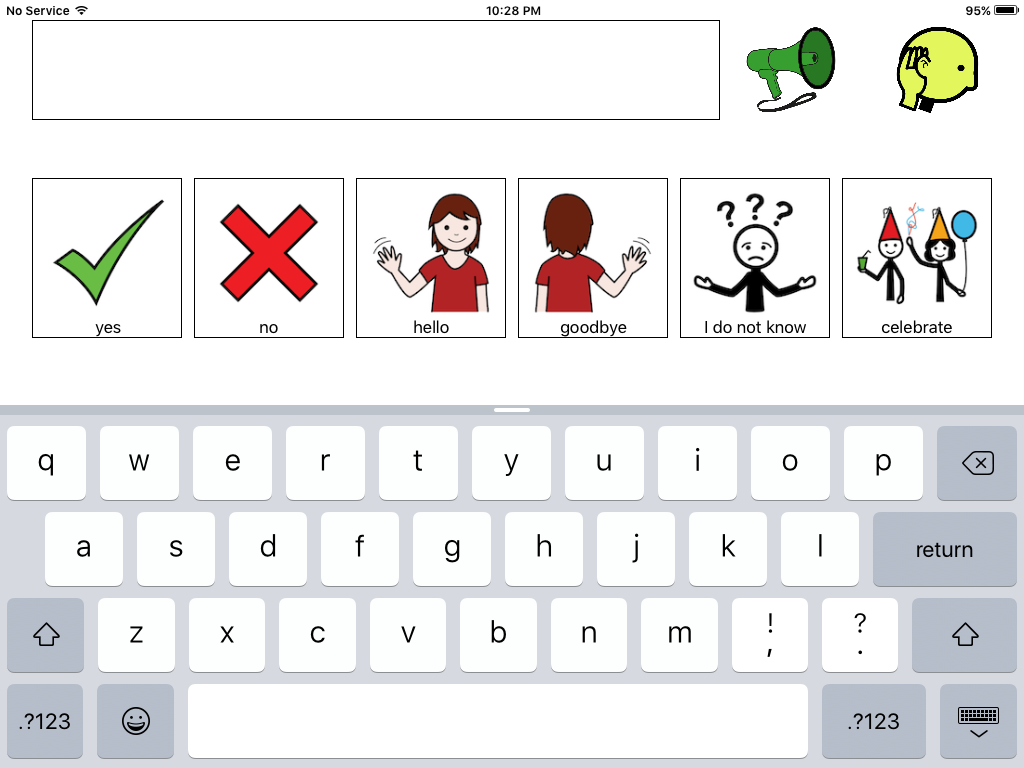
\includegraphics[width=\textwidth]{initialInterface.png}
\caption{Initial Interface on Application Launch}
\label{fig:ui}
\end{figure}

Upon saying the nonverbal user's name, which is programmed into the application on the first launch, or by clicking the listen button, the system will bring up the listening interface, shown in Figure~\ref{fig:listening}, and begin processing verbal input.

\begin{figure}[htb]
\centering
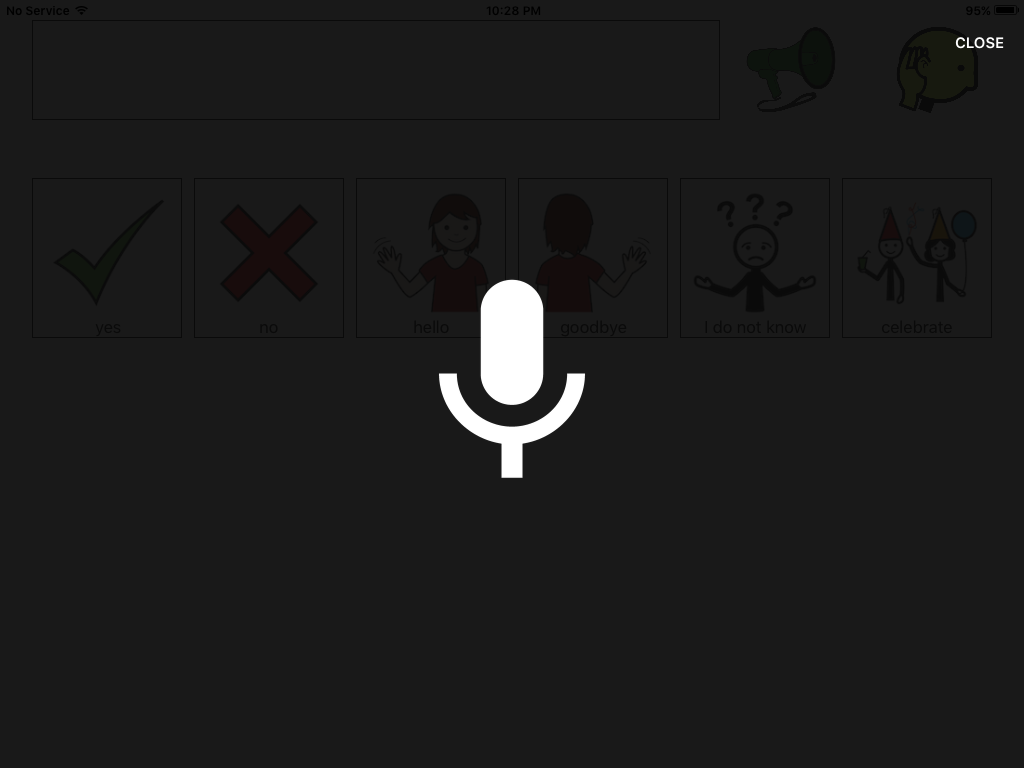
\includegraphics[width=\textwidth]{listeningInterface.png}
\caption{The Listening Interface}
\label{fig:listening}
\end{figure}

When the verbal user is done speaking, the app will finish processing the verbal input and decide which pre-populated category of picture cards to display above the keyboard. Figure~\ref{fig:uiDynamic} shows how the app would adjust if the verbal user said "How do you feel?". 

\begin{figure}[htb]
\centering
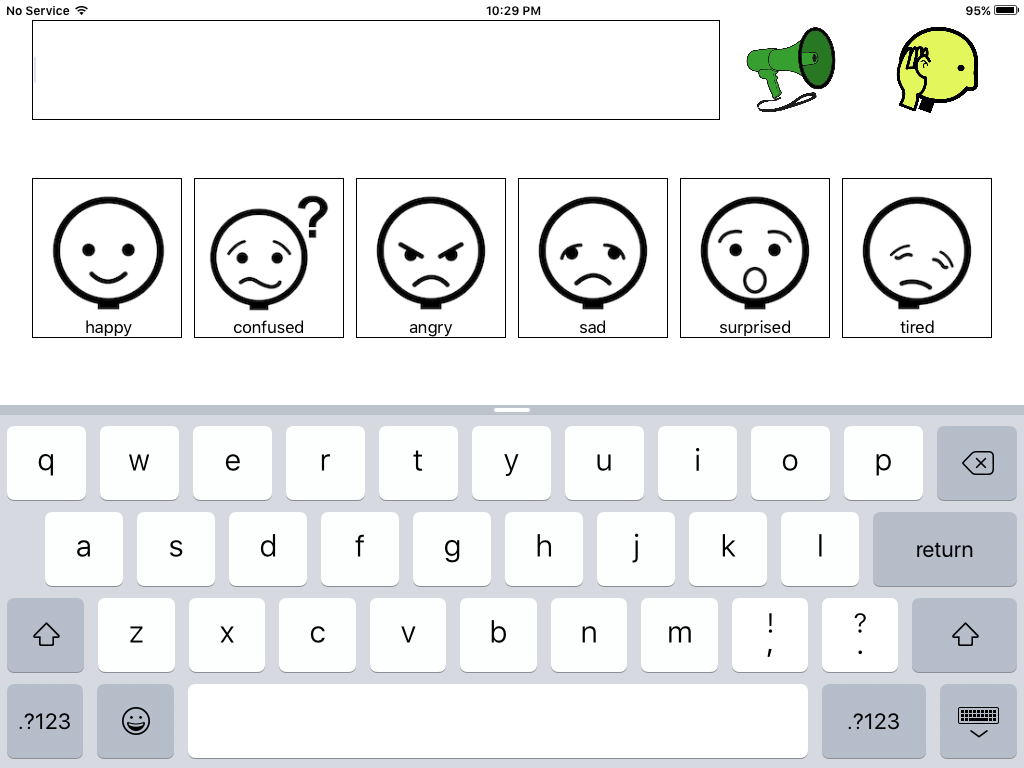
\includegraphics[width=\textwidth]{dynamicInterface.png}
\caption{Demonstration of the Picture Cards adjusting to Dynamic Verbal Input}
\label{fig:uiDynamic}
\end{figure}

At any point during the communication process, the nonverbal user can either press one of the picture cards to immediately speak the word or phrase beneath the card, or press the button on the right of the screen, which will speak what they have typed into the input box aloud.